\subsection{Programmierung des Mikrocontrollers}
\label{kapitel_programmierungMikrocontroller}
 
\subsubsection{Benötigte Software}

Zur Programmierung des Mikrocontrollers mussten zuerst notwendige Software und Treiber geladen und installiert werden.

\begin{description}
	\item[Entwicklungsumgebung:] Arduino IDE (1.6.8), für die Programmierung des Arduino Chip ATmega328, der auf dem Adafruit Pro Trinket verbaut ist
	\item[Bootloader:] Innerhalb der Arduino IDE muss der Bootloader Adafruit AVR Boards (1.4.7) installiert werden
	\item[Treiber für die Adafruit Module:] Adafruit\_driver, Adafruit\_9DOF, \\ Adafruit\_BluefruitLE\_nRF51, Adafruit\_Sensor, Adafruit\_LSM303LHC, \\ Adafruit\_L3GD20\_U, Adafruit\_BMP085\_Unified
\end{description}

Adafruit stellt außerdem über Google Play die Android-App ,,Adafruit Bluefruit LE Connect'' zur Verfügung, über die mit Hilfe der beigefügten Testbeispiele in den Treiberpacketen der Mikrocontroller mit dem Smartphone verbunden und ausprobiert werden kann. 

Für das Projekt wurde eine eigene Android-App entwickelt, die in Kapitel \ref{AndroidAppFürDatenmessen} beschrieben wird.

\subsubsection{Programmieren des Mikrocontrollers}
% setup, loop()
Da der Adafruit Pro Trinket keinen seriellen Ausgabeport hat, wurde die Programmierung zuerst auf einen Arduino Uno geladen, der wie auf der linken Seite der Abbildung \ref{fig:k3_prototyping} mittels eines Breadboards mit den Adafruit-Modulen verbunden war. Während der Programmierung konnte mit \texttt{Serial.print()}-Befehlen der Programmablauf auf dem Mikrocontroller kontrolliert werden, bis er anschließend mit dem gewünschten Verhalten auf den Adafruit Pro Trinket übertragen werden konnte.

Das finale Programm besteht aus zwei Dateien. Nach dem ersten Testlauf wurde der Programmcode des Mikrocontrollers nochmals überarbeitet und auch die Android-App zum Datenempfang (siehe Kapitel \ref{AndroidAppFürDatenmessen}) dazu angepasst. Die Datei \texttt{BluefruitConfig.h} beinhaltet die Belegungen der verwendeten Pinouts des Mikrocontrollers zu den funktionalen Anschlüssen der anderen Modulen. Der eigentliche Programmcode befinden sich in der \texttt{Program.ino}, die im nachfolgenden grob erklärt wird.

Zunächst werden Bibliotheken für die Adafruit Module eingebunden, sowie eine Instanz erstellt, die eine Bluetooth Low Energy-Verbindung aufbaut. Nun gibt es eine \texttt{Setup()}-Funktion, die nur einmal beim Start des Mikrocontrollers aufgerufen wird. Hier wird eine Bluetooth-Verbindung mit einem Smartphone hergestellt und die Sensoren initialisiert. Danach folgt die \texttt{Loop()}-Funktion, die wiederholt aufgerufen wird. Da diese auch auf die gesendeten Befehle der Android-App reagieren muss, wird der Ablauf der Funktion mittels Struktogramm in Abbildung \ref{fig:k3_loopstructo} veranschaulicht.

\begin{figure}[h]
	\centering
	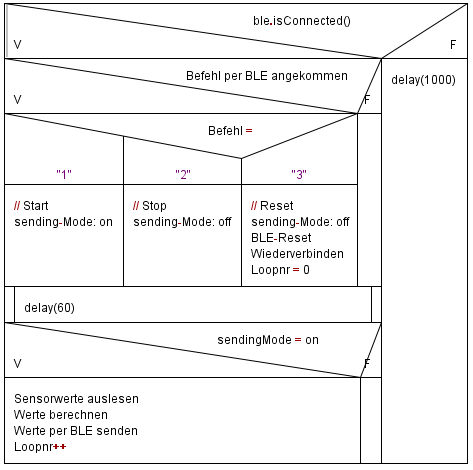
\includegraphics{images/k3-loopstructo.png}
	\caption {Struktogramm des Codeinhaltes der \texttt{Loop()}-Methode}
	\label{fig:k3_loopstructo}
\end{figure}

Besteht keine BLE-Verbindung, wartet der Mikrocontroller 1000ms bis er wieder mit dem erneuten Aufruf der Funktion \texttt{Loop()} beginnt. Bei bestehender Verbindung werden zunächst eventuell empfangene Befehle der Android-App ausgewertet. Sollen Daten gesendet werden (\texttt{sending-Mode = on}), wird mit dem Auslesen der Sensor-Werte und dem Senden dieser per BLE fortgefahren. 

